To answer the needs expressed above, we propose an SLA guided, security-aware continuous data provision and integration approach performed within a multi-cloud service oriented environment  (see
%starting from the processing of the query  to the delivery of the results.
Figure~\ref{fig:arch}). In this section, we present  step-by-step data integration process with the implied  SLA categories.

In our context, data are exposed as  a set of data services on different clouds. In our example of MOOC system presented above, several producers will supply equivalent content for a given period of time  that will be chosen with respect to the  preferences expressed by a consumer. 

Given a query $Q_1$ expressed as Datalog-like program or an SQL-like expression, including spatio-temporal attributes and preferences.
For instance, the following query ``\textit{List of English poetry content providers that can provide commented Emily Dickinson poems that are close to my city and that are labelled as experts, where the total cost is not higher to 1 dollar, with using only services that preserve her anonymity}''. 

The abstract Inter-Cloud Layer (ICL) is in charge of delivering a result to the received query. ICL will first identify a set of semantic functionalities that fit the  query and associated services, stored in the service description registry.

Assume that there are four content providers on English poetry that can be queried individually and two hubs that collect information from other sources like social network groups and hash tags.
Hubs will store content about given topics on  English poetry, available from particular producers (e.g., participants of a given course).
We represent these services by { e$_1$, \dots, e$_4$} and {h$_1$} and {h$_2$}. We suppose that hubs will have the same interface as individual service providers.
We also suppose the existence of two free location services exporting the following interface: {loc(IP) $\rightarrow$ $\langle$ X, Y$\rangle$}, meaning that given an IP address it returns a geographic position expressed as a pair of coordinates. 
All these services can potentially be combined for answering queries.


%shows the general architecture of an SLA guided data integration system. 
%It accesses data services which are data providers deployed in a cloud  that provide agreed SLA's. 
%The whole process is monitored to determine whether a computed SLA is being honoured while a query is evaluated. 

%These descriptions are stored in a directory together with meta-data about the way queries are evaluated for producing results. 
%The system uses this information  by query processing and monitoring modules for rewriting queries according to given quality of service (QoS) preferences expressed by a data consumer, for example a user.The following lines describe how this query is evaluated according to our approach. 

\begin{figure*}
\center{
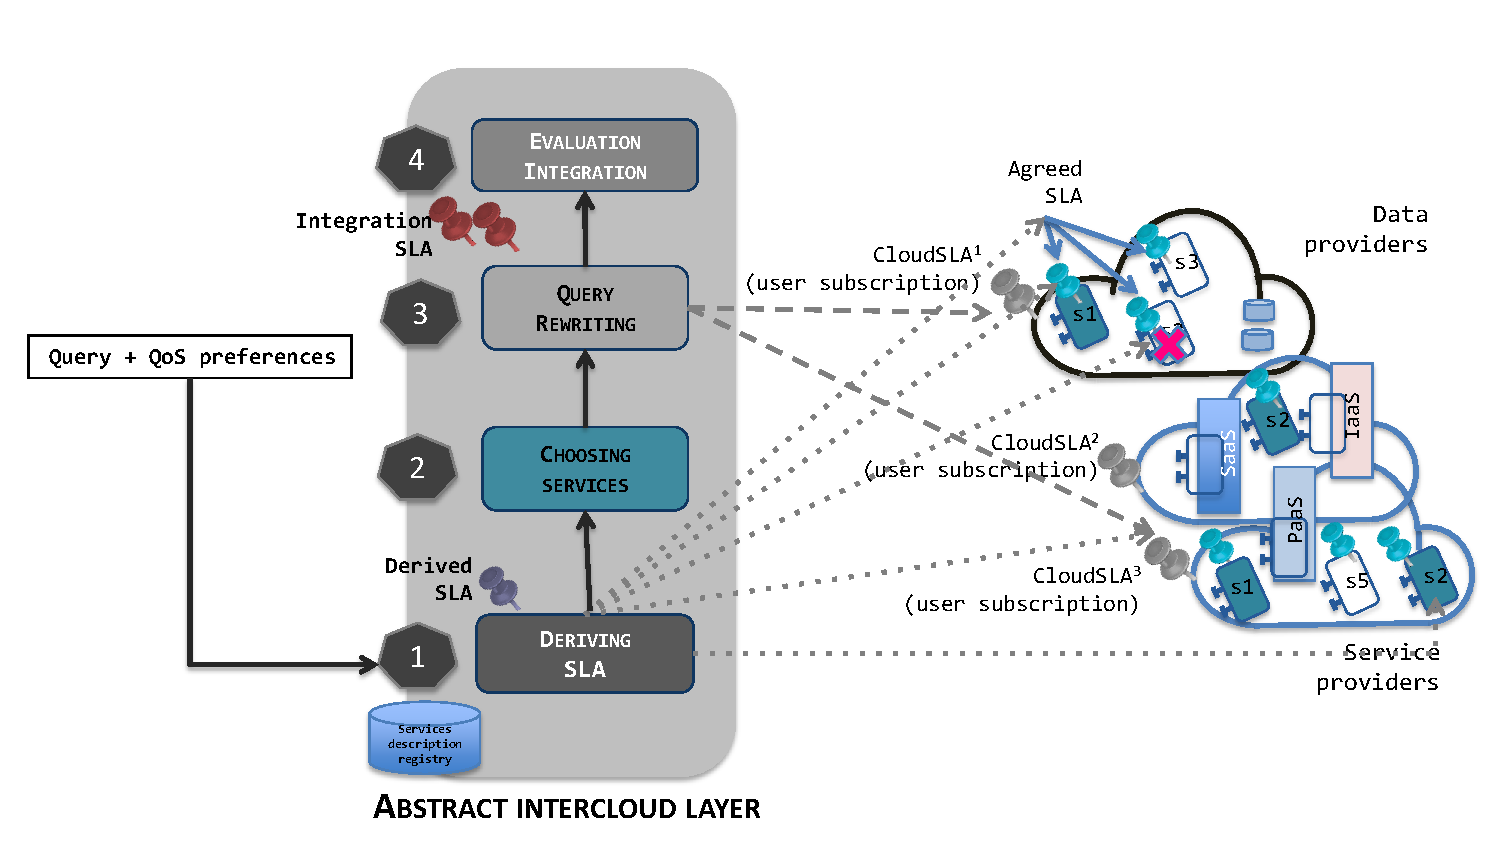
\includegraphics[width=0.75\textwidth]{workflow.pdf}
\caption{Phases of an SLA guided  data integration workflow.\label{fig:arch}}}
\end{figure*}

%In order to illustrate our approach, consider a massive open online course system (MOOC) that aims at being privacy respectful of the students participating in courses and produce and consume content according to the geographic area and expertise of participants. 
%Producers are characterized according to their location, the type and topic of the content that they can provide, the access conditions (e.g. cost, inscription, or exchange unit), and the time window in which they can produce contents. 
%Consumers are described by their location, their interests requirements during a certain interval of time, the maximum total cost they are ready to pay, or the resources they are ready to provide in order to get the service, and quality of service requirements such as availability and how critical it is to consume a given type of content. 
%An energy exchange market is established in order to continuously trade  content provision/consumption ensuring that all consumers will have the content they require at every moment.

Each deployed service exposes an \textit{agreedSLA} that specifies the economic cost per call, the maximum number of calls that can be done per day, the availability of the service, the average response time when a method is called, the reliability, the privacy of the produced data (whether they can be stored or not), the precision, freshness and provenance of the produced data, as defined below:

%NOTE: Agreed SLA are client-provider slas... --MARTIN

\begin{trivlist}\sf\footnotesize
\item[~-~agreedSLA$_i$:] $\langle$cost, availability, freshness, provenance, data access control, certified reputation level, location, duration$\rangle$. 
 \end{trivlist}
 
Some of these measures ({cost/call, maxCall/day}) are static and explicitly specified by the service provider. 
In contrast, the other measures should be computed by monitoring the conversations between the service and the applications that contact it.  It is the case for service reputation that will condition the way personal user data will be anonymized (Constraint1).  Some measures will be instantiated depending on the context of  the service invoked within a multi-cloud environment. It is the case for constraint 2 expressed above:   user data access credentials should be calculated according to the clouds hosting different data services.
An \textit{agreedSLA} is expressed through an  XML document using the specification WSLA (Web service level agreement \footnote{\footnotesize http://www.research.ibm.com/people/a/akeller/\-Data/WSLASpecV1-20030128.pdf}).

Examples of computed measures are the cost of retrieving the list of ``expert'' Emily Dickinson poems providers within a region with their cost. 
The cost is determined by the  cost of the calls. 
This request  includes the price of calling a service (e.g.,  between 0,25 - 0,50 euros depending on the data service), plus the price of data transmission according to the amount of transmitted MegaBytes through the network, the type of subscription of the user for using the network and also the cost of applying encryption algorithm if asked for. The second computed measure is service reputation that is calculated according to the feedback obtained when application contacts the service.




As aforementioned, an a-priori SLA enforcement mechanism is mandatory to assess data integration feasibility.
To this end, non-functional characteristics of the content provision services ({i.e e$_1$, ... e$_4$}) are calculated by specific cloud services (SCS) that enforce SLAs  and which should present an API, composed of a set of methods such as:

 
\begin{trivlist}\sf\footnotesize
\item[~-~]estim-cost$_i$(contents, req\_size, cost, prov\_size, loc), 
%QoS preferences$_\mathit{user}$, -- These should be in the query... not in the concrete services specification.
agreedSLA$_i$.

\item[~-~]engage$_i$(contents, req\_size, payment), agreedSLA$_i$.
\end{trivlist}

 

%Given user expressed QoS preferences ({QoS preferences}$_\mathit{user}$) and {agreedSLA}$_i$, 
The first method allows to obtain for each service $e_i$ the estimation of the budget (in our example, of a given course (content)) and a required minimum size. In other words, it will returns the cost of the data, as well as its actual size and location.
 
The second method is used to engage in a data service (in our example a course data service) and will be used later if the service is retained for a composition that answer the query.

 
%The user will ask for a given derived SLA to which the provider may agree.

ICL by asking SCS for each semantic functionality, obtains the set of potential services that satisfy both user preferences and  service offering described through their \textit{agreed SLAs}. 
Indeed, the query $Q_1$ has two parts: the one that corresponds to the content asked for by the user  that will be solved by combining data services and the \textit{user preferences}, noted by {QoS preferences}$_\mathit{user}$:
\begin{trivlist}\sf\footnotesize
\item[~-~QoS preferences$_\mathit{user}$: ] $\langle$cost, freshness, provenance, location, duration, privacy-preserving$\rangle$. 
\end{trivlist}

 

Let us suppose that for this query the user is ready to pay a maximum of \$1 as total cost; she requests that content providers be certified as experts (provenance) even if their data are not fresh; she requires a contract duration of one week. Besides, she wishes her privacy be saved by adapting the anonymity process with regard to service reputation. The maximum total cost will condition also which kind of privacy preserving algorithms to apply.
 
\begin{trivlist}\sf\footnotesize
\item[~-~QoS preferences$_\mathit{user}$: ] $\langle$cost $\leq$ \$1, freshness = ``any'', provenance = ``certified'', location = ``close'', duration = 7 days, privacy-preserving=``reputation-based''$\rangle$. 
\end{trivlist}



Cloud providers also define their SLA contracts that specify the cost per request ({cost/request}), the volume of data that can be exchanged per month ({I/0 volume/month}), the cost of transferring data or applications within the same data center or between data centers ({datatransferCost/region}), the storage space ({storageSpace}). For example some cloud providers enable the customer to choose the zone to install PaaS services and deploy applications (e.g. zone 1 is Europe). If the customer wishes to deploy services in zone 1 but store data in zone 2 the transfer cost will change.

\begin{trivlist}\sf\footnotesize
 \item[~-~cloudSLA:]  $\langle$cost/request, I/0 volume/month, datatransferCost/region, storageSpace$\rangle$.
 \end{trivlist}
 
Illustration inspired in the lowest contract provided by Azure\footnote{Azure is a trademark of Microsoft Corporation.}: 
 \begin{trivlist}\sf\footnotesize
\item[~-~cloudSLA:]  $\langle$0,05 cents per call, 8 GB I/0 volume/month, free, 1 GB storage$\rangle$. 
\end{trivlist}


 
%A content request is expressed as a query that specifies contents about a given topic with QoS preferences, independently of the possible providers. 

   
 


The next step supervised by the ICL consists in elaborating a set of potential composition specifications via a query rewriting process. Given the user query, specified as a sequence of abstract operations and the available services, specified in the same way, we use a Local-as-View approach~\cite{CostaAMR13} to obtain a combination of services that match the query specification.
The algorithm in~\cite{CostaAMR13} is being modified to deal with agreedSLA and QoS user preferences.

 

In this paper, we are interested in rewritten queries that comply with the QoS user preferences and cloudSLAs.
 This allows computing a result as follows: (i) User preferences (including cloudSLAs according to user subscriptions) and \textit{agreedSLAs} will be used to produce a \textit{derivedSLA} to be associated to the query. These derivedSLA will influence the choice of (data) services that will actually be used for building the result; (ii) Query rewriting for computing service compositions that can be used for  building query results. The \textit{agreedSLA} exposed by the chosen services is added as  conditions in  each re-written query expression; Two situations could arise: a full compliance of a composition with the \textit{derivedSLA} or a partial compliance that requires a negotiation step. For both alternatives, an \textit{integrationSLA} will be produced indicating the negotiation conditions and the implementation of the final integration; (iii) and Managing the integration process according to the \textit{integrationSLA}.

 
%-----------------------------------------------------------------
\section{DerivedSLA}
\label{sec:derivedSla}
%-----------------------------------------------------------------

The key and original aspect of  our proposed data integration and provision process is  defined as a vertical mapping of user QoS preferences and agreedSLAs of potential com posable services. This  leads to a {\em derivedSLA} that guides the evaluation of a query and maps SLA measures and preferences attributes.  

%A query has associated preferences  expressed as macroscopic constraints (i.e. user preferences statement): execution time, pay / no pay, data reliability, provenance, freshness, privacy-preserving constraints, partial/full results, delivery mode. These constraints are coupled with the profile of the user which is in general stated in her cloud subscription (amount of assigned storage space, number of requests, I/O transfered Mega bytes, etc.). 

%As said before, we assume that services export their \textit{agreed SLAs} that define measures that can be either expressed as constants,  computed (dynamically) by monitoring the execution and conversations associated to services, and hybrid they can be statically stated  but they change at execution time.  A service  agreed SLA is expressed through an  XML document using the specification WSLA (Web service level agreement \footnote{\footnotesize http://www.research.ibm.com/people/a/akeller/\-Data/WSLASpecV1-20030128.pdf}). The service SLA measures  that we consider in our example are: cost, availability, freshness, provenance, location, duration of the engagement, privacy-preserving status. Other measures are associated to the conditions in which the service is called or to the precision and recall of their produced data given a request. 


The derivedSLA is defined as a set of measures that correspond to the user preferences computed as a function of different static, computed and hybrid measures. 
The derivedSLA  will guide the way the query will be evaluated, and the way results will be computed and delivered.

In the example, some of the user preferences statement measures are used for defining a derivedSLA that, as said in previous section, will guide the evaluation of the query. 
These measures are defined as a function of the measures used by the agreedSLAs and by the cloud SLA contract. For example: 
\begin{trivlist}\sf\footnotesize
 \item[~-~query total cost:] $\sum_{i = 1\dots n}$ cost(s$_i$) + data transfer + encryption cost $\leq$ \$1.
 \item[~-~availability:] {\em (of services involved)} $\geq$ {\sf 90$\%$}.
 \item[~-~freshness:] non.
 \item[~-~provenance:] all services involved must be $expert$.
 \item[~-~duration:] 7 days.
 \item[~-~I/0 volume/month:] 8GB.
 \item[~-~reputation level :] $\geq$ threshold.
 \item[~-~storageSpace:] 1GB.
 \end{trivlist} 
 
Therefore, we propose a classification of SLA measures that represents the combination of fine grained measures used by agreedSLAs and coarse grained measures used in user preferences statements. 
It specifies also how to compute coarse grained measures with fine grained ones. 
For example, data precision will be computed as a function of availability, freshness and provenance exported by data services. The derivedSLA can be seen as a set of inequations that have to be solved during the execution of a service composition. Since some of them can only be determined at execution time, the decision on which services will participate in the evaluation of the query is approximated.  
This later step may conduct either to the rejection of integration in case of total incompatibility, or to a negotiation step between agreedSLAs and the derivedSLA, which  leads us to the proposal for a negotiated integration SLA  and thus the need for an adaptive setting.
Negotiation of implied SLAs depends strongly on the request sent and the services deployed at the arrival time of the application on the involved  clouds (i.e clouds holding services that satisfies user requests and that are candidate to service composition to answer the query). This negotiation can be expensive and may not scale well.
 
%Given a query and its preferences statement, the system  finds  service compositions that produce results meeting the required constraints, as discussed in the following section.
The resulting derivedSLA will be used in the query rewriting step described in the next section. 
 
%-----------------------------------------------------------------
\section{Query Rewriting}
\label{sec:queryRew}
%-----------------------------------------------------------------

  
 
Query rewriting is a well-known problem in the database domain.
The problem consists in transforming an abstract query into a set (or list) of lower-level queries that can be solved by  available databases.
%Query rewriting is guided by the schema of  abstract and concrete databases.
%The answers to the lower level queries are combined in order to obtain the result to be returned to the user.
The query rewriting problem can be generalized to the case of services.
In this case, the query to be rewritten is seen as an abstract service composition, to be expressed in terms of concrete services.
Query rewriting techniques have been adapted to the context of service composition~\cite{BBM10,ZLC11,CostaAMR13}. 
In~\cite{CostaAMR13} the authors present an algorithm to automatically refine high-level specifications of service compositions into lower-level ones. 
The method is based on the MiniCon algorithm~\cite{PH01} for query rewriting.

The case of more general services (\textit{i.e}, services that maintain and update information) is a generalization of the information-provision case.
Unlike the simpler case, where only the service interfaces need to be considered, the general case requires considering the functional and non-functional aspects of the query and available services.
%In this context, the \textit{Local as View} (\textit{LAV}) methods of query rewriting~\cite{Levy2000} are suitable.
%In the LAV approach, 
The rewriting process is guided by the specification of both the query to be rewritten and the available services.
%The specification of the composition to be produced as well as the specification of each available service are used in the case of general services.
%These specifications may detail both the functional and non-functional behaviour of each service, including SLA.


We propose an approach that consists in generating translations of an abstract query into \textit{several}  compositions over concrete  services. 
%The solutions proposed are ranked and may be coded into concrete workflows as shown in the following section.  
The next example shows the main features of the approach proposed in~\cite{CostaAMR13} which is extended to the case of SLA-guided service-based data integration. 

%\begin{example}[Service Refinement by Rewriting]\label{Ex:rew1}
Let us consider the MOOC scenario, where people can participate on an content trading pool.
We suppose that this hypothetical MOOC has a large number of participants that sell their content  to  consumers. 
The MOOC has four information hubs described by their agreedSLAs, located in four different geographic locations, connected to other content providers.
These laters may be  contacted directly, through the services of three different cloud providers that exposes their CloudSLA.
 
  

When an on-line consumer searches servers to buy/retrieve content, a composed web service is generated, in order to fetch each individual or hub service and to start  content retrieval procedures.
Depending on the location of the consumer and producers, different conditions and constraints may apply.
Also  cloud providers  publish the conditions for using their services.
These conditions and non-functional requirements (such as authentication or security requirements) should also been expressed in the QoS user preferences and agreedSLAs.

In this context, the user  expresses a content order, her location and payment information. A composite web service is  generated to fulfill the order.
The generated service composition should consider the nearest providers, in accordance to the agreedSLA.

In order to produce a personalized service composition for each user, the algorithm in~\cite{CostaAMR13} takes into account the specification of the composition. The specification of each available service is also considered is given. 
%~\hfill\openbox
%\end{example}

 
%Given a set of services that can possibly be composed and the derived SLA, a service composition must be produced.
%Some of the inequations of the derived SLA should be included in the service compositions that answers the query.

The agreedSLA will be included and merged with the SLA conditions obtained by the rewriting process. Only those compositions that comply with the agreedSLA will be presented as possible solutions to the user.
 

In the case of our query example the following composition can be used for answering it:

\begin{footnotesize}
\sf
\begin{tabbing}
 -~Q(myIPad\=dress, ``E.Dickinson'', 1MB, ``expert'', \$1, myCreditCard) $\equiv$ \\
 \>  myLoc = loc(myIPaddress), \\
 \>  estim$\_$cost(``E.Dickinson'', 1MB, cost, size, theirLocation), \\
 \>  query total cost + cost $\leq$ \$1,\\
 \>  availability $\geq$ 90$\%$, \\
 \>  freshness = any, \\
 \>  provenance = ``expert'', \\
 \>  duration = 7 days, \\
 \>  I/0 volume/month $\leq$ 8GB, \\
 \>  reputation level $\geq \lambda$ (the threshold) \\
 \>  storageSpace $\leq$ 1GB, \\
 \>  engage(``E.Dickinson'', size, myCreditCard).
 \end{tabbing} 
\end{footnotesize}

Our approach would generate a number $k$ of service compositions, combining as much as possible the services available such that the constraints of the derivedSLA are verified. 
 Yet, the algorithm should be modified to take into account the different SLAs. 
 
%-----------------------------------------------------------------
\section{Towards an integration SLA}
\label{sec:queryProcessOpt}
%-----------------------------------------------------------------
 Our data provision and integration approach relies on data services deployed on one or different clouds providers and it is delivered as a distributed DaaS on top of the clouds involved.  This DaaS  uses resources from a cloud and this use  is  guided by an economic model (stated in a cloud subscription) that puts a threshold on the amount of resources to be invested in a query evaluation process. It is thus important to optimize the use of these resources. 
   
The optimization of this process can occur at two levels: first at the level of agreedSLA exported by services.  Indeed, queries requesting the same services compositions will have clauses in their SLAs that are more conditions of use of the infrastructure (ie not storing the data produced by a service). Instead of recomputing the derivedSLA every time, we propose to store it and reuse it for other queries. 
Second, pre-computed queries and partial results can be also stored in cache or in a persistent support. Rewriting results can be also stored and reduce execution and resources consumption time when evaluating similar queries. Storing or not such SLAs will depend on the cloud subscription of the user the issued the query (data access, intermediate storage capacity , cost of storage , etc ... ).


Furthermore, the way the integration will take place after the choice of the concrete service composition will require to enforce functional and non functional user and service preferences to take into account the integration constraints. In the example this has been illustrated by  the access control level constraints demanded by data services when they are implied in an integration process. Another important point is to consider the existing inter-cloud contracts as described in \cite{} to decide how to implement the integration it self. This leads to the build of the \textit{integration SLA} 
 

%As discussed in previous sections, the derived SLA associated to service compositions can have free measures that can only be evaluated at run-time. In order to do so, we assume that there is a monitoring system observing and aggregating events for computing resources consumption, execution and time cost, volumes of data transferred when services deliver results. These computations are used dynamically for instantiating free variables in the derived SLA and thus determine whether the contract is respected by the execution of a query. Since this is monitored dynamically, the evaluation of the query can be adapted if the SLA is not being respected anymore.
%
 


